\newpage
\section{Auswertung}
\label{sec:Auswertung}

Die in \autoref{sec:Auswertung} gezeigten Grafiken und Ausgleichsrechnungen sind mithilfe der Python-Bibliotheken Matplotlib \cite{matplotlib}, Scipy \cite{scipy} und Numpy \cite{numpy}
erstellt worden.
Da die Grad-Skala immer den doppelten Wert aufzeigt, wird in \autoref{sec:Auswertung} immer
die Hälfte des Werts auf der Skala genommen.
\subsection{Überprüfung der Bragg-Bedingung}

Wie in der Durchführung beschrieben wird ein fester Kristallwinkel von $\Theta = 14°$
eingestellt. 
\begin{figure}[H]
  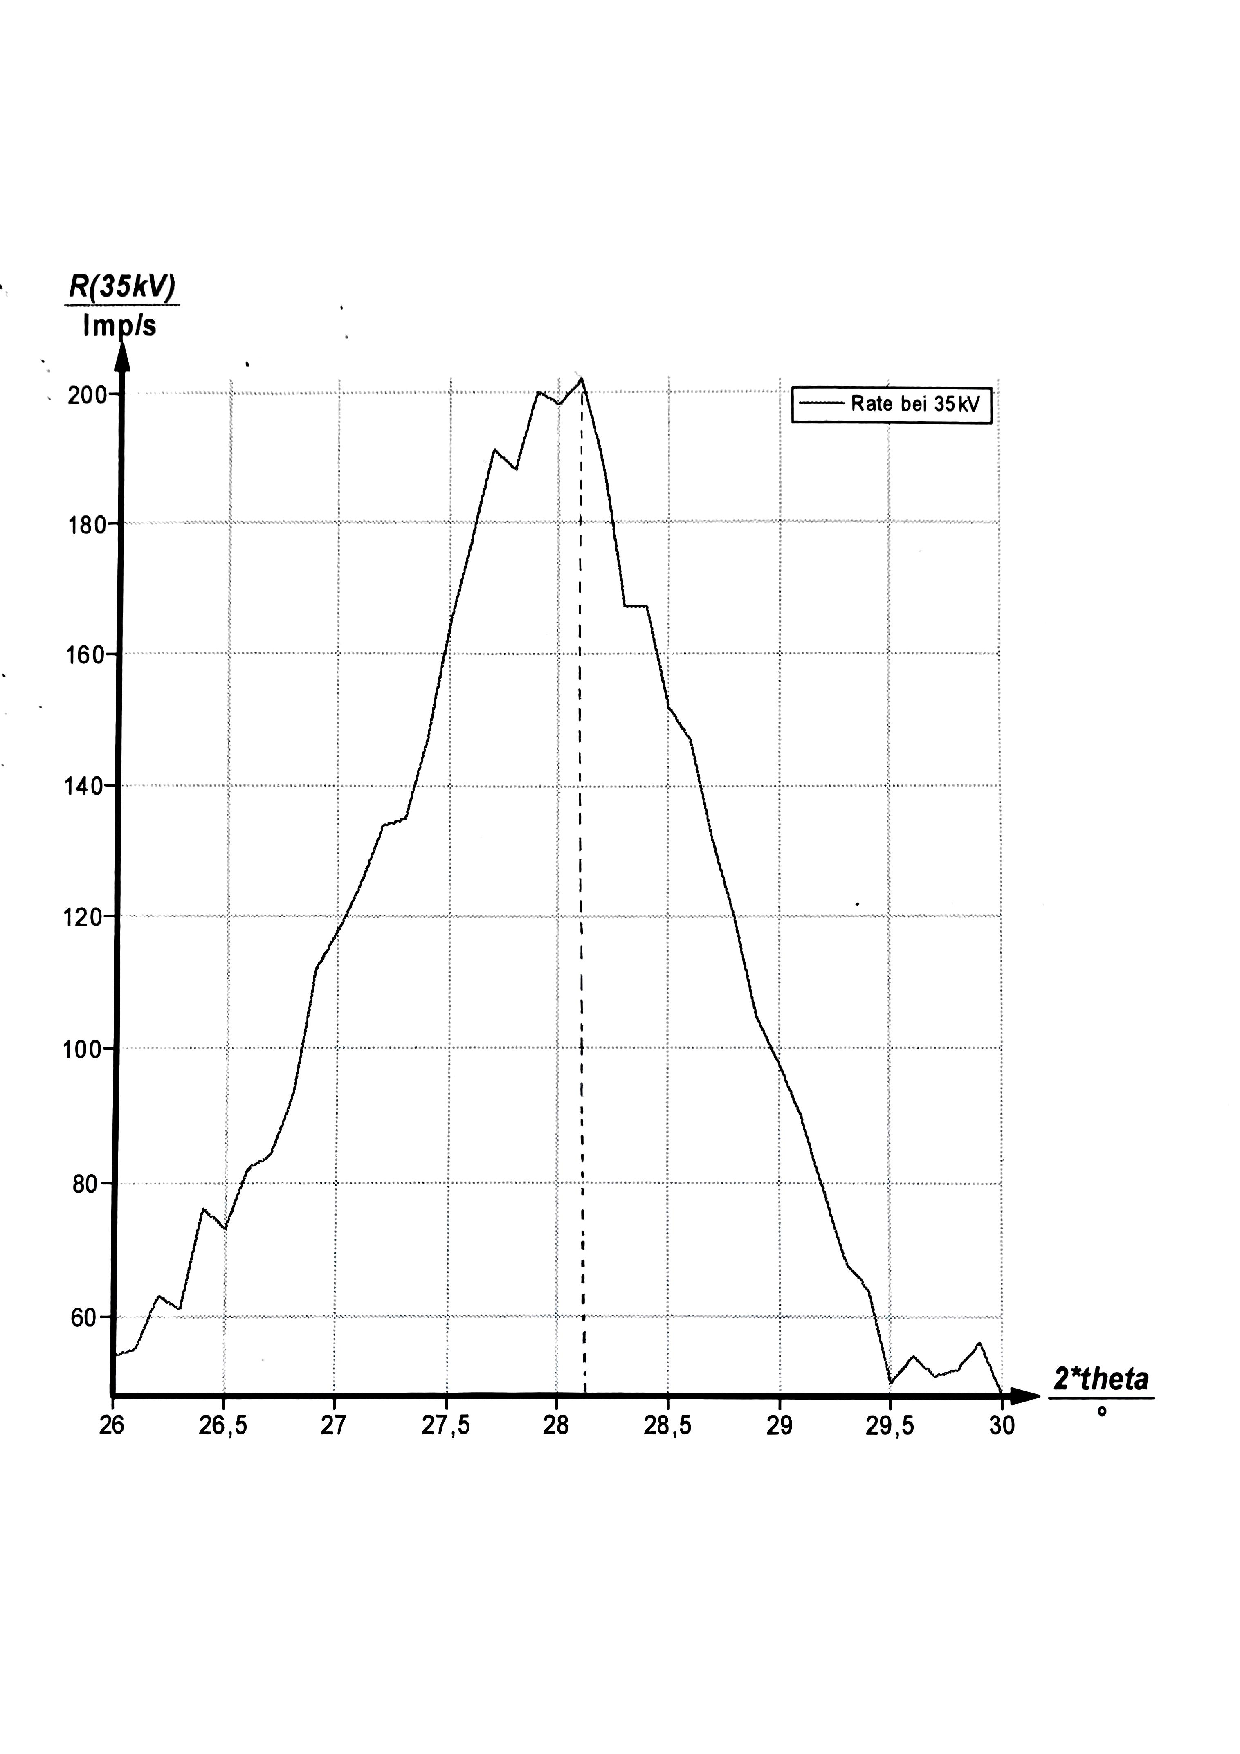
\includegraphics[width=\linewidth, height=14cm]{build/braggbedingung.pdf}
  \caption{Messergebnisse der ersten Versuchsreihe und erwartetes Maximum.}
  \label{fig:braggbedingung}
\end{figure}
Das Maximum der Kurve lässt sich aus \autoref{fig:braggbedingung} bei
\begin{equation*}
  \Theta_{max} = \SI{14.05(0.05)}{°}
\end{equation*}
ablesen und beträgt
\begin{equation*}
  R_{max} = \SI{203(1)}{Imp/s}.
\end{equation*}

\subsection{Das Emissionsspektrum einer Cu-Röntgenröhre}
\begin{figure}[H]
  \includegraphics[width=\linewidth, height=14cm]{build/bremsberg.pdf}
  \caption{Emissionsspektrum einer Cu-Röntgenröhre.}
  \label{fig:spektrum}
\end{figure}

In \autoref{fig:spektrum} ist der Bremsberg gekennzeichnet. Die K-Linien lassen sich in \autoref{fig:detail} bei 
\begin{align*}
  \Theta_{\beta} &= \SI{20.2(0.1)}{°} \\
  \text{und }\Theta_{\alpha} &= \SI{22.5(0.1)}{°}
\end{align*}
ablesen.
\begin{figure}[H]
  \includegraphics[width=\linewidth, height=14cm]{build/detail.pdf}
  \caption{Detailspektrum der $K_{\alpha}-$ und $K_{\beta}-$Linie.}
  \label{fig:detail}
\end{figure}
Mit \autoref{eq:lambda_min} und \autoref{eq:Energie_Photon} ergibt sich für die frei werdende Energie
\begin{align*}
  E_{\alpha} &= \SI{8044(34)}{eV} \\
  \text{und }E_{\beta} &= \SI{8915(40)}{eV}.
\end{align*}
Die Halbwertsbreiten sind in \autoref{fig:detail} ablesbar (siehe \autoref{eq:detail}) und betragen umgerechnet in Energien
\begin{align*}
  H_{\alpha} &= \SI{169}{eV} \\
  \text{und }H_{\beta} &= \SI{191}{eV}.
\end{align*}
\begin{align}\label{eq:detail}
  \beta_1 &= \SI{20.4(0.1)}{°}\\
  \beta_2 &= \SI{19.9(0.1)}{°}\\
  \alpha_1 &= \SI{22.7(0.1)}{°}\\
  \alpha_2 &= \SI{22.2(0.1)}{°}.
\end{align}

Damit ergeben sich die Auflösungsvermögen nach \autoref{eq:Spektrales_Aufloesungsvermoegen}
\begin{align*}
  A_{\alpha} &= \SI{42(13)}{}\\
  \text{und }A_{\beta} &= \SI{53(15)}{}.
\end{align*}
Mit \autoref{eq:sig} lassen sich die Abschirmkonstanten bestimmen
\begin{align*}
  \sigma_1 &= 3.3\\
  \sigma_2 &= \SI{12.42(0.30)}{}\\
  \sigma_3 &= \SI{22.5(2.2)}{}.
\end{align*}
Dabei wurde die Absorptionsenergie $E_{abs} = \SI{8.9789}{keV}$ aus entsprechender Literatur entnommen \cite{E_abs}.

\subsection{Untersuchung des Absorptionsspektrums}
In \autoref{fig:k-kanten} sind die Ausschläge des Geiger-Müller-Zählrohrs bei Verwendung verschiedener Absorber-Materialien dargestellt. 
Die eingezeichneten K-Kanten sind näherungsweise auf die Mitte der Kante gelegt. Mit \autoref{eq:lambda_min}, \autoref{eq:Energie_Photon} 
und \autoref{eq:sig} folgt
\begin{table}
  \centering
  \begin{tabular}{c c c c c}
      \toprule
      {} & {$Z$} & {$E_{K}\left[\unit{keV}\right]$} & {$\Theta_{K}\left[\unit{°}\right]$} & {$\sigma_{K}$}\\
      \midrule
      Zn & 30 & $\SI{8.98(0.04)}{}$  & $\SI{20.1(0.1)}{}$ & $\SI{4.31(0.06)}{}$ \\
      Br & 35 & $\SI{13.48(0.10)}{}$ & $\SI{13.2(0.1)}{}$ & $\SI{3.52(0.12)}{}$ \\
      Sr & 38 & $\SI{16.06(0.14)}{}$ & $\SI{11.1(0.1)}{}$ & $\SI{3.64(0.15)}{}$ \\
      Zr & 40 & $\SI{17.73(0.18)}{}$ & $\SI{10.0(0.1)}{}$ & $\SI{3.90(0.18)}{}$ \\
      \bottomrule
  \end{tabular}
  \caption{Ergebnisse für Energie und Abschirmkonstante.}
  \label{tab:1}
\end{table}

\begin{figure}[H]
  \centering
  \begin{subfigure}[b]{0.49\textwidth}
      \centering
      \includegraphics[width=\textwidth, height=10cm]{build/zink.pdf}
      \caption[]
      {{\small Zink-Absorber.}}    
      \label{fig:zn}
  \end{subfigure}
  \hfill
  \begin{subfigure}[b]{0.49\textwidth}  
      \centering 
      \includegraphics[width=\textwidth, height=10cm]{build/brom.pdf}
      \caption[]
      {{\small Brom-Absorber.}}    
      \label{fig:br}
  \end{subfigure}
  \vskip\baselineskip
  \begin{subfigure}[b]{0.49\textwidth}   
      \centering 
      \includegraphics[width=\textwidth, height=10cm]{build/strontium.pdf}
      \caption[]
      {{\small Strontium-Absorber.}}    
      \label{fig:sr}
  \end{subfigure}
  \hfill
  \begin{subfigure}[b]{0.49\textwidth}   
      \centering 
      \includegraphics[width=\textwidth, height=10cm]{build/zirkonium.pdf}
      \caption[]
      {{\small Zirkonium-Absorber}}    
      \label{fig:zr}
  \end{subfigure}
  \caption[ The average and standard deviation of critical parameters ]
  {\small K-Kanten verschiedener Absorber.} 
  \label{fig:k-kanten}
\end{figure}

\subsection{Bestimmung der Rydbergenergie}
Nach Moseley ist die Absorptionsenergie $E_K$ proportional zum Quadrat der Ordnungszahl $Z$. Mit diesem Zusammenhang ist es möglich die 
Rydbergenergie $R_{\infty}$ durch eine Ausgleichgerade der Form 
\begin{equation*}
  \sqrt{E} = a \cdot Z + b
\end{equation*}
zu bestimmen. Mit den Ordnungszahlen und den zuvor berechneten Energien aus \autoref{tab:1} ergeben sich durch eine Ausgleichsrechnung mit der Python 
Funktion curve fit \cite{scipy}
\begin{align*}
  a &= \SI{3.86(0.17)}{\sqrt{eV}}\\
  \text{und } b &= \SI{-20.32(6.13)}{\sqrt{eV}}.
\end{align*}
Mit $R_{\infty} = a^{2}$ folgt für die Rydbergenergie
\begin{equation*}
  R_{\infty} = \SI{14.9(0.03)}{eV}.
\end{equation*}
\begin{figure}[H]
  \includegraphics[width=\textwidth]{build/rydberg.pdf}
  \caption{Ergebnisse aus \autoref{tab:1} und Ausgleichgerade.}
\end{figure}